
\documentclass[12pt,table,a4paper]{report}
\usepackage{lmodern}
\usepackage[utf8]{inputenc}
\usepackage[T1]{fontenc}
\usepackage{fancyhdr}
\usepackage[french]{babel}
\usepackage[none]{hyphenat}
\usepackage{listings}
\usepackage[nottoc,numbib]{tocbibind}
\usepackage{todonotes}
\usepackage{amssymb}
\usepackage{footmisc}

\title{TFE: Plateforme de ticketing}
\author{Emmanuel CAPELLE}
\date{}

\DeclareUnicodeCharacter{00A0}{ }
\pagestyle{fancy}
\lhead{}
\renewcommand{\rmdefault}{phv}
\renewcommand{\sfdefault}{phv}
\renewcommand{\headrulewidth}{0.4pt}
\renewcommand{\footrulewidth}{0.4pt}
% \setcounter{secnumdepth}{2} % only chapter and sections will be numbered
% \setcounter{tocdepth}{4}    % entries down to \subsubsections in the TOC
\setlength{\parindent}{0pt}

\begin{document}

\maketitle

\newpage

\tableofcontents

\newpage

\chapter{Introduction}

\section{État de la question}
Le sujet que je vais aborder dans ce travail de TFE sera la “Conception d’une plateforme de gestion de services d’assistance”.

Il existe sur le web plusieurs solutions, appelées “systèmes de ticketing”, qui répondent à la demande de logiciel de gestion de services d’assistance.

Lors de mon stage en entreprise, j’ai eu pour tâche de développer une application web permettant de gérer en ligne des tickets concernant des appartements habités par les utilisateurs de cette plateforme.

Il existe d’autres exemple de plateformes déjà existantes, tel que "Mantis Bug Tracker"\footnote{https://www.mantisbt.org/}, qui se focalise quant à elle sur l’assistance au développement d’applications informatique.

J’ai abordé ce sujet de TFE avec plusieurs problêmes en tête:
\begin{enumerate}
\item{La vitesse d’exécution du framework utilisé lors de mon stage\footnote{YII: http://www.yiiframework.com/} s’avérait être très lent, malgré l’utilisation rigoureuse des best-practices préconisés par les créateurs dudit framework.}
\item{La flexibilité de ces différentes plateformes reste assez limitée, j’aimerais créer une plateforme extensible à souhait, pouvant se "`métamorphoser"' en une plateforme adaptée aux besoins de ses utilisateurs, via une interface administrateur.}
\item{J’aimerais ajouter une capacité d’ubiquité à ma plateforme en lui ajoutant une application Android permettant de créer et/ou gérer des tickets, peu importe la localisation de ses utilisateurs.}
\end{enumerate}


\section{Délimitation du projet}
Le projet est constitué de deux parties: d'une part l'application web qui servira d'interface principale à ses utilisateurs, leur permettra de gérer leur compte utilisateur et les paramètres associés à celui-ci ainsi que la création de tickets directement sur le site.

L'accent sera mis sur la communication entre les différents protagonistes pour la résolution de problèmes des utilisateurs de la plateforme. Les différents protagonistes sont les utilisateurs, les gestionnaires de tickets, et les entreprises susceptibles de pouvoir résoudre le problème lié au ticket.

D'autre part, une application android a été créée en tant que support pour l'application web principale. Sa valeur ajoutée est qu'elle permet aux utilisateurs de créer un ticket où qu'ils soient, sans devoir avoir accès à un ordinateur.

\section{Définition de quelques concepts}
\textbf{Service d'assistance}: service offert par l'entreprise propriétaire de la plateforme pour mettre en relation utilisateurs de ladite plateforme et entreprises étant susceptible de résoudre le problème rencontré par l'utilisateur.

\textbf{Ticket}: Un ticket est une demande d'assistance émise par l'utilisateur de la plateforme. Celui-ci est ensuite pris en charge par un gestionnaire de ticket, qui servira d'intermédiaire entre l'utilisateur et une ou plusieurs entreprises.

\textbf{Administrateur}: Dans le cas de cette application, l'administrateur est la/les personnes en charge du backend de l'application. (Base de données, code, ...)

\textbf{Gestionnaire de tickets}: La ou les personne(s) chargée(s) de donner suite aux demandes d'assistance (tickets) émises par les utilisateurs sur la plateforme.

\textbf{Utilisateur}: Est un utilisateur «lambda» de la plateforme, n'ayant aucune permission spéciale dans le système.

\textbf{Django}: Le framework utilisé pour construire la nouvelle plateforme de ticketing.


\chapter{Approche théorique et technique}
\section{Outils et méthodes utilisés}
Environnements de travail:

Développement du site web: IDE PyCharm – community edition de JetBrains.\footnote{https://www.jetbrains.com/pycharm/}

Développement de l'app Android: Android studio de JetBrains.\footnote{http://developer.android.com/tools/studio/index.html}

\section{Langage de programmation utilisé: Python}
Créé en 1990 par Guido van Rossum, Python est un langage de programmation de haut niveau à typage dynamique, orienté objet et est un langage interprété, plutôt que compilé.

Ce langage à l'avantage d'être portable, et peut fonctionner sur quasiment toutes les systèmes d'exploitation disponibles sur le marché. Si j'ai envie de porter mon application de ticketing sur linux, il est tout à fait possible de le faire, et ce assez facilement.

Python est aussi un langage qui a pris beaucoup de maturité, ce qui a pour avantage d'avoir une assez grande communauté, et par conséquent un choix de librairies assez conséquent.

Simple et direct, Python est particulièrement bien adapté au dévelopement rapide d'applications (RAD).

Il est possible aussi d'interfacer python avec d'autres langages comme C++, java, c\#, etc... Son utilisation est alors plus orientée vers le scripting de comportements.

Pourquoi ai-je choisi Python? 

Je connais bien Python en tant que langage de programmation. Je l'utilise souvent pour créer des scripts de tout type. C'est un langage très flexible et adaptable à de nombreuses situations.

C'est pourquoi j'ai voulu approfondir ma connaissance de ce langage en lui découvrant une nouvelle facette: La programmation web.

\section{Le framework utilisé: Django}
Django est un framework orienté web créé en Python.

Ce framework permet le développement non seulement rapide, mais aussi modulaire d'applications web, enlevant à cette occasion la nécéssité de "réinventer la roue".

Pourquoi Django?

Dans le domaine des frameworks web pour développement rapide de sites web, Django a beaucoup de concurrence (CodeIgniter, Laravel, Yii, ruby on rails, ASP.NET,... Pour ne citer que quelques uns des frameworks les plus connus dans le milieu).

Dans un contexte de popularité du framework par rapport à ses concurrents, Django se place dans le haut du classement (Au moment de l'écriture de ce rapport).\footnote{http://hotframeworks.com/\#top-frameworks}

Il existe de nombreuses offres d'emploi requérant la connaissance de Django, certes, pas autant que d'autres frameworks tel que ASP.NET, mais Django se place de manière très respectable sur le marché du travail.

Finalement, j'ai choisi Django car j'ai voulu apprendre une nouvelle manière de développer une application web.

\subsection{Fonctionnement de Django}
\subsubsection{Déploiement rapide d'application}
Le déploiement d'une application Django requiert deux choses:

\begin{itemize}
	\item{Une distribution python correctement installée, et préférablement dans sa version 3.x vu les performances améliorées dans cette nouvelle version}
	\item{Les dépendances de librairies python, facilement installées grâce à l'outil PIP qui installe Django et ses dépendances en une seule commande console.}
\end{itemize}

Après avoir installé python, la librairie Django et ses dépendances, il ne reste qu'à soit cloner un projet Django depuis votre hébergeur git, mercurial ou autre, soit créer un nouveau projet Django.

Django utilise son propre serveur web, pas besoin d'apache pour livrer les pages web aux utilisateurs de la plateforme.

\subsubsection{Architecture web découplée}
Django à comme spécificité d'être modulable à l'extrème. En effet, il est très facile avec ce framework de pouvoir ajouter un nouveau module à la volée, et avec un minimum de configuration.

La seule exigence du framework est que l'application web doit posséder un module de base, standardisé, et créé d'office lors de la création de l'application web via Django-admin (voir chapitre précédent).

Ce système apporte beaucoup de choses bénéfiques au développement web, et la non-nécéssité de devoir "réinventer la roue" à chaque démarrage de projet.

Ce système, très efficace, permet le développement de "plugins"\footnote{Plugin : Extension d'une application principale pour en étendre les fonctionnalités.} et une utilisation rapide de ceux-ci dans des applications existantes.
Par exemple, il est possible qu'une entreprise ai créé son propre système de login sécurisé et réutilisable, il lui est donc très facile d'intégrer ce module dans un projet déjà existant, permettant ainsi de développer plus rapidement de nouveaux modules.

\subsubsection{Architecture MVC}
À vrai dire, les développeurs de Django appellent l'architecture utilisée par Django "`architecture MTV"' (Model-Template-View) qui, selon leur dires \footnote{https://docs.djangoproject.com/en/1.8/faq/general/ : "`Django appears to be a MVC framework, but you call the Controller the 'view', and the View the 'template'. How come you don’t use the standard names?"'}, diffère par le fait que la vue "décrit quelles données l'on voit, et non pas comment celles-ci sont visibles".

La vue est, somme toute, un fonction appelant un template. La vue passe alors des données au template, qui lui se chargera de les représenter "graphiquement" à l'écran pour l'utilisateur final.

Personnellement, je n'ai pas trouvé cette architecture différente de celle utilisée par MVC, il existe juste cette subtilité décrite ci-dessus, qui ne change au final pas grand chose dans le workflow de développement du site web.

Qu'est-ce que MVC?

Cette architecture sépare l'application en trois grandes parties, le modèle qui s'occupe de la partie applicative logique, ainsi que des interactions entre la base de données et l'application.

La vue quant à elle sert à définir l'interface homme-machine de l'application, qui permettra à ses utilisateurs de consulter et d'interagir avec les données de l'application.

Pour terminer, le contrôlleur, qui s'occupe de la gestion et de la validation des interactions faites par les utilisateurs via les vues de la plateforme.

Il est à noter que Django utilise une nomenclature propre pour désigner les différentes parties du modèle MVC: Le modèle s'appelle toujours modèle, par contre la vue s'appelera "template", et le contrôleur s'appellera "views", pour cause, le fichier s'occupant de la partie contrôlleur de l'application s'appelle... "views.py". C'est d'ailleurs ce que j'ai trouvé déroutant lorsque j'ai découvert le framework.

\subsubsection{Les modèles}
Les modèles en Django sont tous contenus dans un fichier appelé "models.py". Ce fichier existe dans chacuns des modules existant dans l'application Django.

Les modèles sont représentés par une classe. Ces classes sont consituées de champs (primary key, foreign key, champs normaux,...), mais aussi de méthodes définissant le comportement du modèle, et qui seront appelées par les contrôleurs afin de pouvoir travailler, modifier ou supprimer ces objets.

La création d'objets se fait dans le contrôleur. (voir section sur les contrôleurs, plus bas)

Chacune des classes modèle dérive d'une classe "`Model"' parente, contenant tous les comportements de base d'un modèle. Par exemple: sauvegarde de l'objet dans la DB (via l'ORM), suppression d'un objet, entre autres.

Tous ces comportements sont bien entendu redéfinissables afin de se comporter de la manière la plus adaptée aux besoins du développeur, et donc ultimement aux besoins des utilisateurs.

Il est par exemple possible de redéfinir la méthode "`delete()"' dans le but de passer un champ "`visible"' à faux, au lieu de supprimer la donnée de la base de données. Cette technique est appelée "`soft delete"', et je l'utilise dans mon application.

Cette méthode de découpe des modèles en classes python permet aussi une certaine facilité dans l'écriture de bateries de tests, j'y reviendrai un peu plus tard dans la section consacrée aux tests.

\subsubsection{Les vues}
Il y a deux façons d'aborder la création de vues avec Django:

\begin{itemize}
	\item{Vues fonctionnelles: la vue est alors créée sous la forme d'une fonction, retournant une URL pointant vers un template à faire apparaître à l'écran.}
	\item{Classes vue: La vue est une classe dérivant de la classe parente "TemplateView", la vue devient alors un objet python à part entière, et son comportement peut-être modifié via la redéfinition des méthodes de la classe parente.}
\end{itemize}

Étant donné que les vues dites "fonctionnelles" sont plutôt adaptées aux petits sites web, j'ai choisi d'utiliser exclusivement les classes de vue. En effet, elles donnent accès à l'avantage certain de la flexibilité possible uniquement avec l'orienté objet.

\subsubsection{Comment ces vues fonctionnent-elles?}

Chaque classe de vue est couplée à un template. La différence entre la vue et le template est que la vue se charge de communiquer les données entre le ou les modèle(s) et le template. La fonction de la classe de vue est finalement celle d'un contrôleur normal dans une architecture MVC.

Pour que les utilisateurs puissent atteindre les différentes vues qui composent la plateforme, il est nécéssaire de les lier à une URL unique, c'est alors que le "routeur", aussi appelé "URL dispatcher".

Il existe dans le module racine un routeur de base contenant les instructions de routage de base. L'URL passe d'abord par ce premier routeur qui s'occupe, lui, d'importer la partie de site web requise par l'URL.

Voici le routeur "racine" utilisé par mon application web:
\begin{figure}
	\centering
		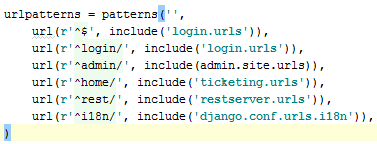
\includegraphics[width=0.8\textwidth,natwidth=377,natheight=144]{images/ticket-routeur-racine.png}
	\caption{Exemple de routeur racine}
	\label{fig:ticket-routeur-racine}
\end{figure}

Les autres modules contiennent aussi un routeur, secondaire celui-ci, qui se charge de déterminer le endpoint\footnote{Endpoint: Destination finale à atteindre \label{endpointFootnote}} à atteindre. Une fois cet endpoint\footref{endpointFootnote} déterminé, la vue passe par la méthode d'appel adéquate (GET ou POST), passe les données nécéssaires au template, s'il y en a, qui, lui, affichera la page finale dans le navigateur de l'utilisateur.

Voici à quoi ressemble un routeur secondaire:
\begin{figure}
	\centering
		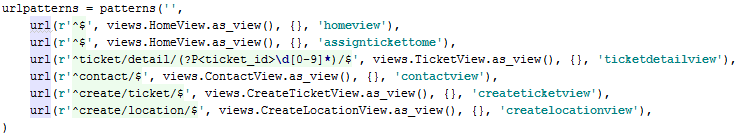
\includegraphics[width=0.8\textwidth,natwidth=737,natheight=136]{images/ticket-routeur-secondaire.png}
	\caption{Exemple de routeur secondaire}
	\label{fig:ticket-routeur-secondaire}
\end{figure}


\todo{TODO: Les vues}

\subsubsection{Les contrôleurs}
\todo{TODO: Les contrôleurs}

\subsection{L'ORM de Django}
\todo{TODO: L'ORM de Django}
Après avoir écrit les classes modèles, il faut traduire lesdites classes en tables et champs dans la/les base(s) de données utilisée(s) par l'application.

\subsection{SQLite versus MySQL}
SQLite est un type de base de données léger, stocké dans un fichier ".db", ce qui rend cette base de données portable: Un simple copier-coller la relocalise. C'est une très bonne base de données pour tester les applications en développement.

Cependant, SQLite ne possède aucun système de gestion des utilisateurs SQL, de fait il n'y a qu'un seul utilisateur, en tout et pour tout, pouvant effectuer des opérations sur la base de données SQLite.

Cela veut donc dire, aucune connection concurrente possible, et donc perte de performances lors de l'accès à la DB, que ce soit en lecture ou en écriture.

Il est donc sage de penser à la migration depuis une base de donnée type SQLite vers une base de données MySQL, celle-ci prenant en charge la concurrence de plusieurs connections simultannées à ses tables.


\chapter{Implémentation des différentes applications}

\section{Solution de gestion des tickets existante}

\subsection{Présentation du système de ticketing}
Cette plateforme de ticketing a été réalisée lors de mon stage en entreprise.

Son utilité principale consiste en la mise en relation de différents protagonistes pour la résolution de problèmes présents sur le lieu d'habitation des utilisateurs de cette plateforme.

Son implémentation a été pensée de telle sorte que l'utilisateur de la plateforme puisse trouver une entreprise susceptible de pouvoir résoudre son problème.

\subsection{Structure organisationnelle de l'application}
\todo{TODO: structure organisationnelle de l'application (YII)}

\subsection{Critique de la plateforme existante}
Cette plateforme ne se basait que sur des catégories et sous-catégories d'incidents, et souvent, une entreprise assignée à tel incident se trouvait beaucoup plus loin géographiquement qu'une autre entreprise pouvant résoudre le même type de problème.

De plus, les performances au niveau de la vitesse d'exécution de la plateforme laissait à désirer, il fallait souvent attendre plusieurs secondes avant de pouvoir accéder à la page web désirée.

Finalement, l'architecture mise en place côté plateforme web nous a bloqué lorsque le client nous a demandé de développer un webservice, dans le but de créer une application Android travaillant de paire avec le site web.

\section{Conception de la nouvelle solution}
C'est avec les différents problèmes énoncés lors de la section précédente en tête que je me suis mis à développer un système de ticketing et son application Android, tout en utilisant une approche différente de celle adoptée lors de mon stage en entreprise.

\subsection{Business rules}
Il est nécéssaire dans ce genre d'applications travaillant avec divers acteurs, qui eux-mêmes travaillent en harmonie pour atteindre un objectif commun (la résolution de problèmes de particuliers), de définir des règles métiers qui assureront le bon fonctionnement de l'application.

Voici les principales règles métier mises en place:

\subsubsection{Administration de la plateforme}
\begin{itemize}
	\item{L'administrateur de la plateforme pourra choisir s'il est possible pour les utilisateurs de la plateforme de s'enregistrer manuellement sur ladite plateforme. Objectif: Filtrage d'éventuelles création de compte intempestive.}
\end{itemize}

\subsubsection{Gestion des tickets}
\begin{itemize}
	\item{Une fois la création d'un ticket effectuée, la gestion de celui-ci sera entièrement donnée au gestionnaire de ticket. Il sera cependant possible pour l'utilisateur de communiquer avec son gestionnaire de ticket via la section commentaire dudit ticket, ou via la fonctionnalité de contact disponible sur la page principale "`Home"' de la plateforme.}
\end{itemize}

\subsection{Flux d'information}
Je vais diviser cette section en deux parties distinctes, car il existe deux flux distincts d'informations: Le flux d'information interne au site web, et celui utilisé par l'application Android via le webservice implémenté aux côtés du site web.

\subsubsection{Flux d'information du site web}
\todo{Flux d'information site web}

\subsubsection{Flux d'information entre le webservice et l'application Android}
\todo{Flux d'information android}

\subsection{Analyse UML de l'application conçue}
\todo{Analyse UML de la plateforme}
\missingfigure{UML}

\subsection{La base de données utilisée par les applications}

\subsubsection{Dictionnaire de données}
Cette partie va vous présenter les différentes données utilisées dans la base de données unique de l'application.
\todo{dictionnaire de données}

\subsubsection{Schéma de la base de données}
\todo{Schéma de la BDD}

\section{Analyse de l'application Android}

\subsection{Pourquoi une application Android?}
\todo{Pourquoi une application android?}
Dans un monde où la population bouge beaucoup, il est important pour une application de pouvoir être disponible n'importe où, et à n'importe quel moment.

Cette application permet aux utilisateurs de la plateforme de pouvoir gérer et être mis à jour de l'avancement de son ou ses ticket(s) en cours.

\subsection{Flow de l'application Android}
\todo{flow de l'application android}
\missingfigure{Flow app android}
Cette section va parler du flow suivi par un utilisateur et par un gestionnaire lorsqu'il utilise l'application Android.

\subsection{Client REST}
Le client REST est implémenté côté application Android afin de communiquer avec un webservice, qui est le plus souvent un serveur REST implémenté à côté d'un site web.
\todo{Analyse client REST}

\subsection{Mise en place d'un bus d'évènements}
\todo{Analyse bus d'évènements}

\chapter{Conclusion}
\todo{conclusion}
J'ai énormément appris lors de mon stage, ainsi que lors de l'implémentation de ce site web et de son application Android.

Je n'avais jamais essayé d'implémenter un site web en python, ni implémenté de web service. Android était aussi pour moi une grande inconnue.

\begin{thebibliography}{breitestes Label}
	\bibitem{How to tango with Django}
	site web: http://en.wikibooks.org/wiki/LaTeX/List\_Structures
	
	\bibitem{Documentation Django online}
		site web: https://docs.djangoproject.com/en/1.8/
\end{thebibliography}

\end{document}
